\chapter{IMPLEMENTASI DAN PENGUJIAN SISTEM}
\label{chap:implemtasiPL}

Bab ini membahas implementasi serta pengujian dari aplikasi {data capture} berbasis Node.js sebagai bentuk perwujudan dari rancangan sistem sebelumnya. Penjelasan pada bab ini mencakup realisasi tampilan antarmuka perangkat lunak, simulasi operasional sistem ketika memproses input data secara langsung, serta rangkaian pengujian sistem secara komprehensif. Simulasi dan pengujian tersebut secara spesifik mendemonstrasikan bagaimana sistem memvalidasi fungsionalitas, mengintegrasikan model pembelajaran mesin, serta merespons dan membedakan antara input data penyewa yang berstatus aman dengan penyewa yang berpotensi melanggar.

% Sub-bab 5.1 Tampilan Perangkat Lunak
\section{Tampilan Perangkat Lunak}

Pada bab ini akan membahas antarmuka pengguna (\textit{user interface}) dari aplikasi {Data Capture}. Aplikasi ini dirancang untuk memfasilitasi proses pencatatan data penyewa, peninjauan data yang telah tersimpan, serta pembaruan informasi secara dinamis. Hak akses aplikasi dibedakan menjadi dua peran (\textit{role}) utama, yaitu Pengelola dan Pelaku Komersil. Rincian fungsionalitas dan tampilan dari setiap halaman aplikasi dipaparkan sebagai berikut.

\subsection{Halaman \textit{Login}}
Halaman {login} berfungsi sebagai antarmuka autentikasi awal bagi seluruh pengguna. Pada tahap ini, pengguna diwajibkan untuk memasukkan {e-mail} dan kata sandi (\textit{password}).

\begin{figure}[H]
    \centering
    \includegraphics[width=0.85\textwidth]{Gambar/login (sementara).png}
    \caption{Tampilan Halaman \textit{Login}}
    \label{fig:ui_login}
\end{figure}

\subsection{Halaman Daftar}
Halaman pendaftaran (\textit{register}) disediakan secara khusus bagi pengguna dengan peran Pelaku Komersil yang belum memiliki akun, sehingga mereka dapat mendaftarkan diri secara mandiri. Sementara itu, akun dengan peran Pengelola tidak dapat mendaftar melalui halaman ini karena akun Pengelola akan didaftarkan langsung oleh administrator.

\begin{figure}[H]
    \centering
    \includegraphics[width=0.85\textwidth]{Gambar/daftar (sementara).png}
    \caption{Tampilan Halaman Pendaftaran Akun}
    \label{fig:ui_daftar}
\end{figure}

\subsection{Halaman \textit{Dashboard}}
Halaman {dashboard} merupakan antarmuka utama yang ditampilkan setelah pengguna berhasil masuk (\textit{login}) ke dalam aplikasi. Tampilan dan informasi pada halaman ini disesuaikan dengan hak akses dari masing-masing peran pengguna.

Bagi pengguna dengan peran Pengelola, halaman {dashboard} menyajikan data statistik penyewa secara keseluruhan, mencangkup seluruh aktivitas transaksi yang dilakukan oleh semua Pelaku Komersil. Selain itu, Pengelola juga memiliki wewenang khusus untuk mengunggah atau melakukan perubahan terhadap Laporan Pelanggaran mencangkup foto dan deskripsi pelanggarannya. Laporan yang telah diunggah tersebut kemudian dapat dilihat oleh seluruh pengguna aplikasi.

Sementara itu, bagi pengguna dengan peran Pelaku Komersil, data statistik yang ditampilkan pada {dashboard} dibatasi hanya pada rekapitulasi data penyewaan dari akun miliknya sendiri. Terkait fitur Laporan Pelanggaran, Pelaku Komersil hanya memiliki hak akses untuk melihat laporan yang telah dipublikasikan oleh Pengelola dan tidak memiliki kewenangan untuk mengunggah laporan pelanggaran.

\begin{figure}[H]
    \centering
    \includegraphics[width=0.85\textwidth]{Gambar/dashboard sesudah.png}
    \caption{Tampilan Halaman {Dashboard}}
    \label{fig:ui_dashboard}
\end{figure}


\subsection{Halaman Input}
Halaman \textit{input} didesain untuk mengakomodasi proses rekam data penyewa baru ke dalam basis data aplikasi. Struktur antarmuka pada halaman ini bersifat seragam untuk kedua peran pengguna. Fokus fungsionalitasnya ditujukan untuk mengumpulkan formulir yang mencakup informasi profil identitas penyewa beserta rincian detail transaksi sewanya.

\begin{figure}[H]
    \centering
    \includegraphics[width=0.85\textwidth]{Gambar/input sesudah.png}
    \caption{Tampilan Halaman Input Pengelola}
    \label{fig:ui_input_Pengelola}
\end{figure}

\begin{figure}[H]
    \centering
    \includegraphics[width=0.85\textwidth]{Gambar/input sesudah.png}
    \caption{Tampilan Halaman Input Pelaku Komersil}
    \label{fig:ui_input_Pelaku_Komersil}
\end{figure}

\subsection{Halaman Lihat / Edit Data}
Halaman ini memungkinkan pengguna meninjau ulang riwayat data penyewa yang telah tersimpan, sekaligus melakukan pencatatan informasi pelengkap seperti pencatatan waktu keluar (\textit{check-out}) atau modifikasi metode pembayaran dan jenis sewa. Berikut antarmuka yang dibedakan berdasarkan peran yang diembannya.

\begin{figure}[H]
    \centering
    \includegraphics[width=0.85\textwidth]{Gambar/lihat edit data sesudah.png}
    \caption{Tampilan Halaman Lihat / Edit Data Pengelola}
    \label{fig:ui_lihat_edit_data_Pengelola}
\end{figure}

\begin{figure}[H]
    \centering
    \includegraphics[width=0.85\textwidth]{Gambar/lihat edit data sesudah.png}
    \caption{Tampilan Halaman Lihat / Edit Data Pelaku Komersil}
    \label{fig:ui_lihat_edit_data_Pelaku_Komersil}
\end{figure}

Berikut adalah rincian fitur pada halaman Lihat / Edit Data yang dibagi berdasarkan masing-masing peran.
\begin{itemize}
    \item \textbf{Pengelola:} memiliki kewenangan akses secara menyeluruh. Pengelola berhak meninjau semua rekam data penyewaan yang terdaftar di dalam aplikasi. Melalui halaman ini, Pengelola dapat melengkapi jam \textit{check-out}, memodifikasi metode pembayaran, mengubah jenis sewa, serta melakukan \textit{checklist} pada bagian komentar apabila ditemukan indikasi pelanggaran. Tanda \textit{checklist} ini dapat dibiarkan kosong apabila tidak ditemukan indikasi pelanggaran. Selain itu, Pengelola juga dapat mengunduh (\textit{download}) seluruh data penyewa beserta detail riwayat aktivitasnya (\textit{log}), memverifikasi keberadaan data ganda (\textit{duplicate}), serta menyaring tabel (\textit{filter}) agar hanya menampilkan data penyewa yang terindikasi memiliki pelanggaran. Selain itu, halaman ini juga menyediakan fungsionalitas untuk penyegaran data tabel (\textit{refresh}) dan fitur pencarian informasi spesifik (\textit{search}).
    
    \item \textbf{Pelaku Komersil:} memiliki ruang lingkup kewenangan yang dibatasi. Pengguna dengan peran ini hanya diizinkan untuk mengakses dan meninjau data penyewa yang didaftarkan oleh akunnya sendiri. Pelaku Komersil diberikan hak pembaruan yang sama—seperti menginput waktu \textit{check-out}, memperbarui metode pembayaran, memodifikasi jenis sewa, dan menandai \textit{checklist} komentar pelanggaran (dibiarkan kosong jika tidak terdapat pelanggaran)—namun tindakan tersebut hanya berlaku secara spesifik terhadap data penyewa kepemilikannya. Otoritas pengunduhan data beserta rincian \textit{log}-nya juga dibatasi ketat pada rekam data yang berada di bawah otoritas operasionalnya. Meski demikian, fitur navigasi dasar seperti penyegaran tabel (\textit{refresh}) dan fungsi pencarian data (\textit{search}) tetap dapat diakses secara penuh.
\end{itemize}

\subsection{Halaman Manajemen Unit}
Halaman Manajemen Unit difungsikan sebagai pusat pengelolaan data untuk menambahkan atau mengurangi daftar unit penyewaan yang dimiliki oleh setiap Pelaku Komersil. Halaman ini bersifat eksklusif hanya untuk pengguna dengan peran Pengelola.

\begin{figure}[H]
    \centering
    \includegraphics[width=0.85\textwidth]{Gambar/manajemen unit sesudah.png}
    \caption{Tampilan Halaman Manajemen Unit}
    \label{fig:ui_manajemen_unit}
\end{figure}

% Sub-bab 5.2 Simulasi Input Data
\section{Pengujian Sistem}

Subbab ini menguraikan pengujian aplikasi {data capture} serta pengujian skenario peluncuran model (\textit{model deployment}) melalui simulasi penggunaan aplikasi saat pengguna memasukkan data penyewa ke dalam sistem. Untuk membuktikan kapabilitas model klasifikasi yang telah diintegrasikan, pemaparan pada bagian ini difokuskan pada dua skenario utama, yakni simulasi \textit{input} profil data penyewa normal (aman) dan simulasi \textit{input} data penyewa tidak normal (berpotensi melanggar). Secara keseluruhan, simulasi ini ditampilkan untuk memperlihatkan tahapan pengisian formulir pendataan sewa, eksekusi model terintegrasi, hingga munculnya respons prediksi atau notifikasi dari aplikasi sesaat setelah pengguna menyimpan data.

\newpage
\subsection{Skenario Input Data Penyewa Normal}
Skenario pertama mendemonstrasikan proses pendataan untuk penyewa yang memiliki profil dan pola transaksi wajar. Pada tahap ini, pengguna memasukkan identitas penyewa beserta data pendukung terkait transaksi penyewaan.

\begin{figure}[H]
    \centering
    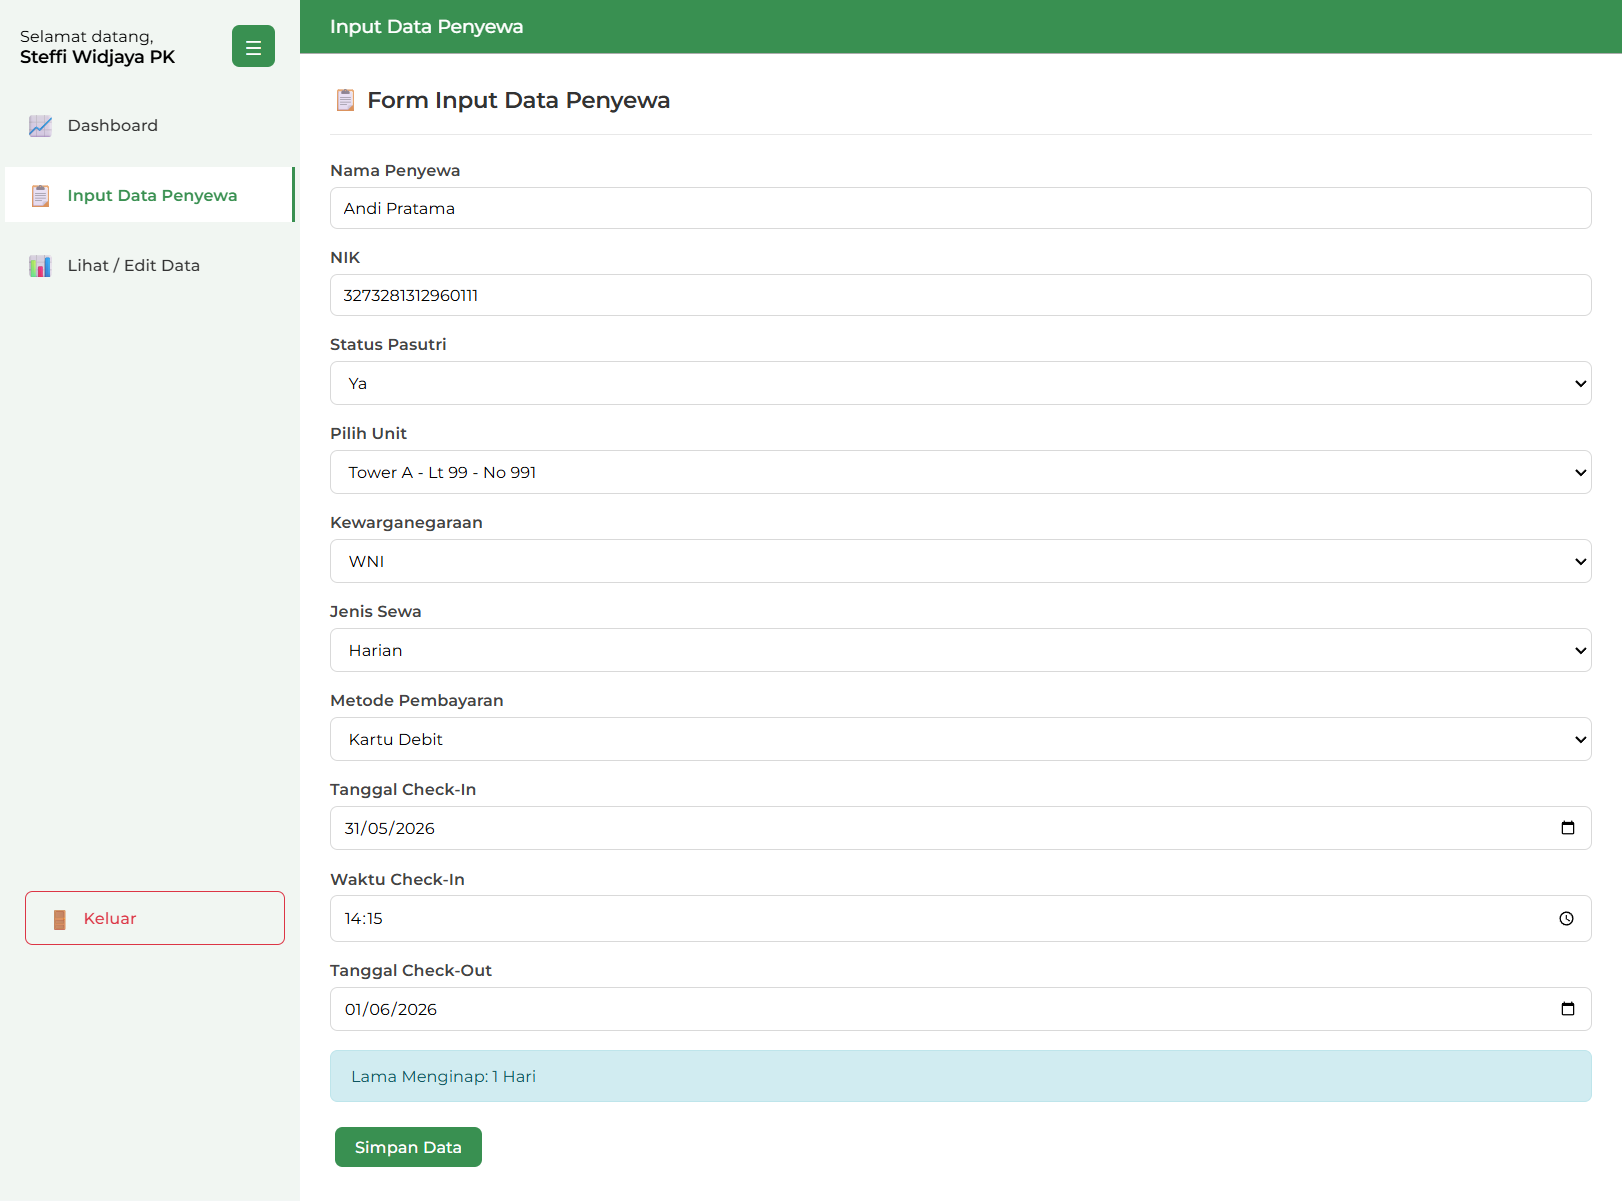
\includegraphics[width=0.7\textwidth]{Gambar/NONmelanggar1a.png} \\
    \vspace{0.2cm}
    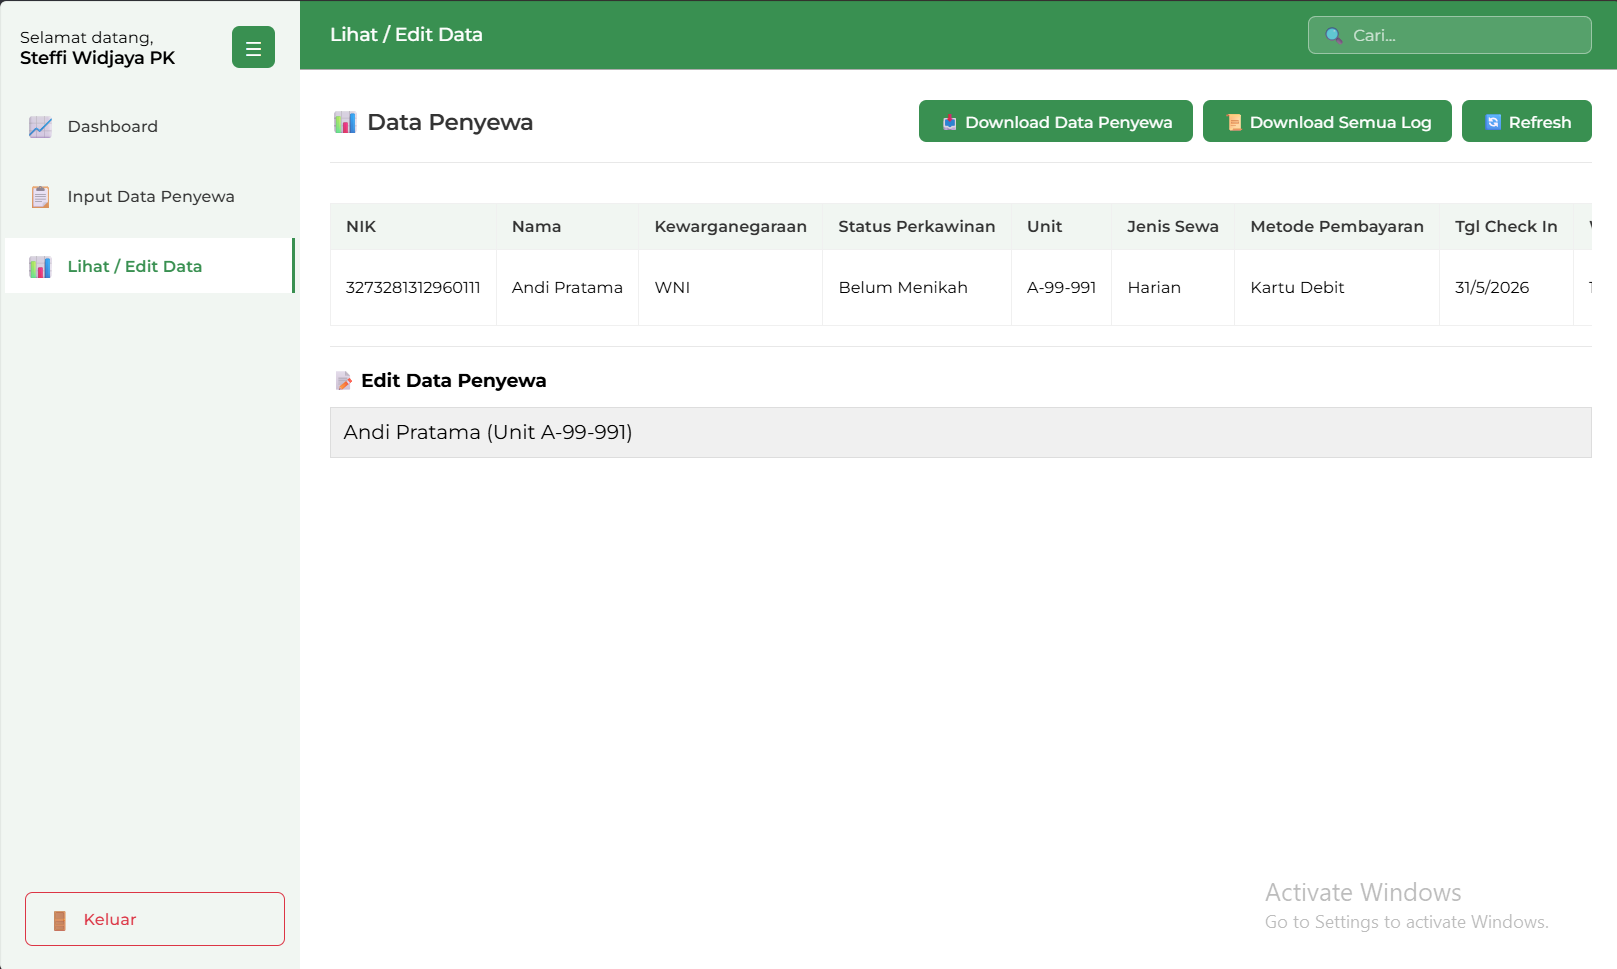
\includegraphics[width=0.7\textwidth]{Gambar/NONmelanggar1b.png}
    \caption{Simulasi Input Data Penyewa Normal (1)}
    \label{fig:sim_input_normal1}
\end{figure}

\begin{figure}[H]
    \centering
    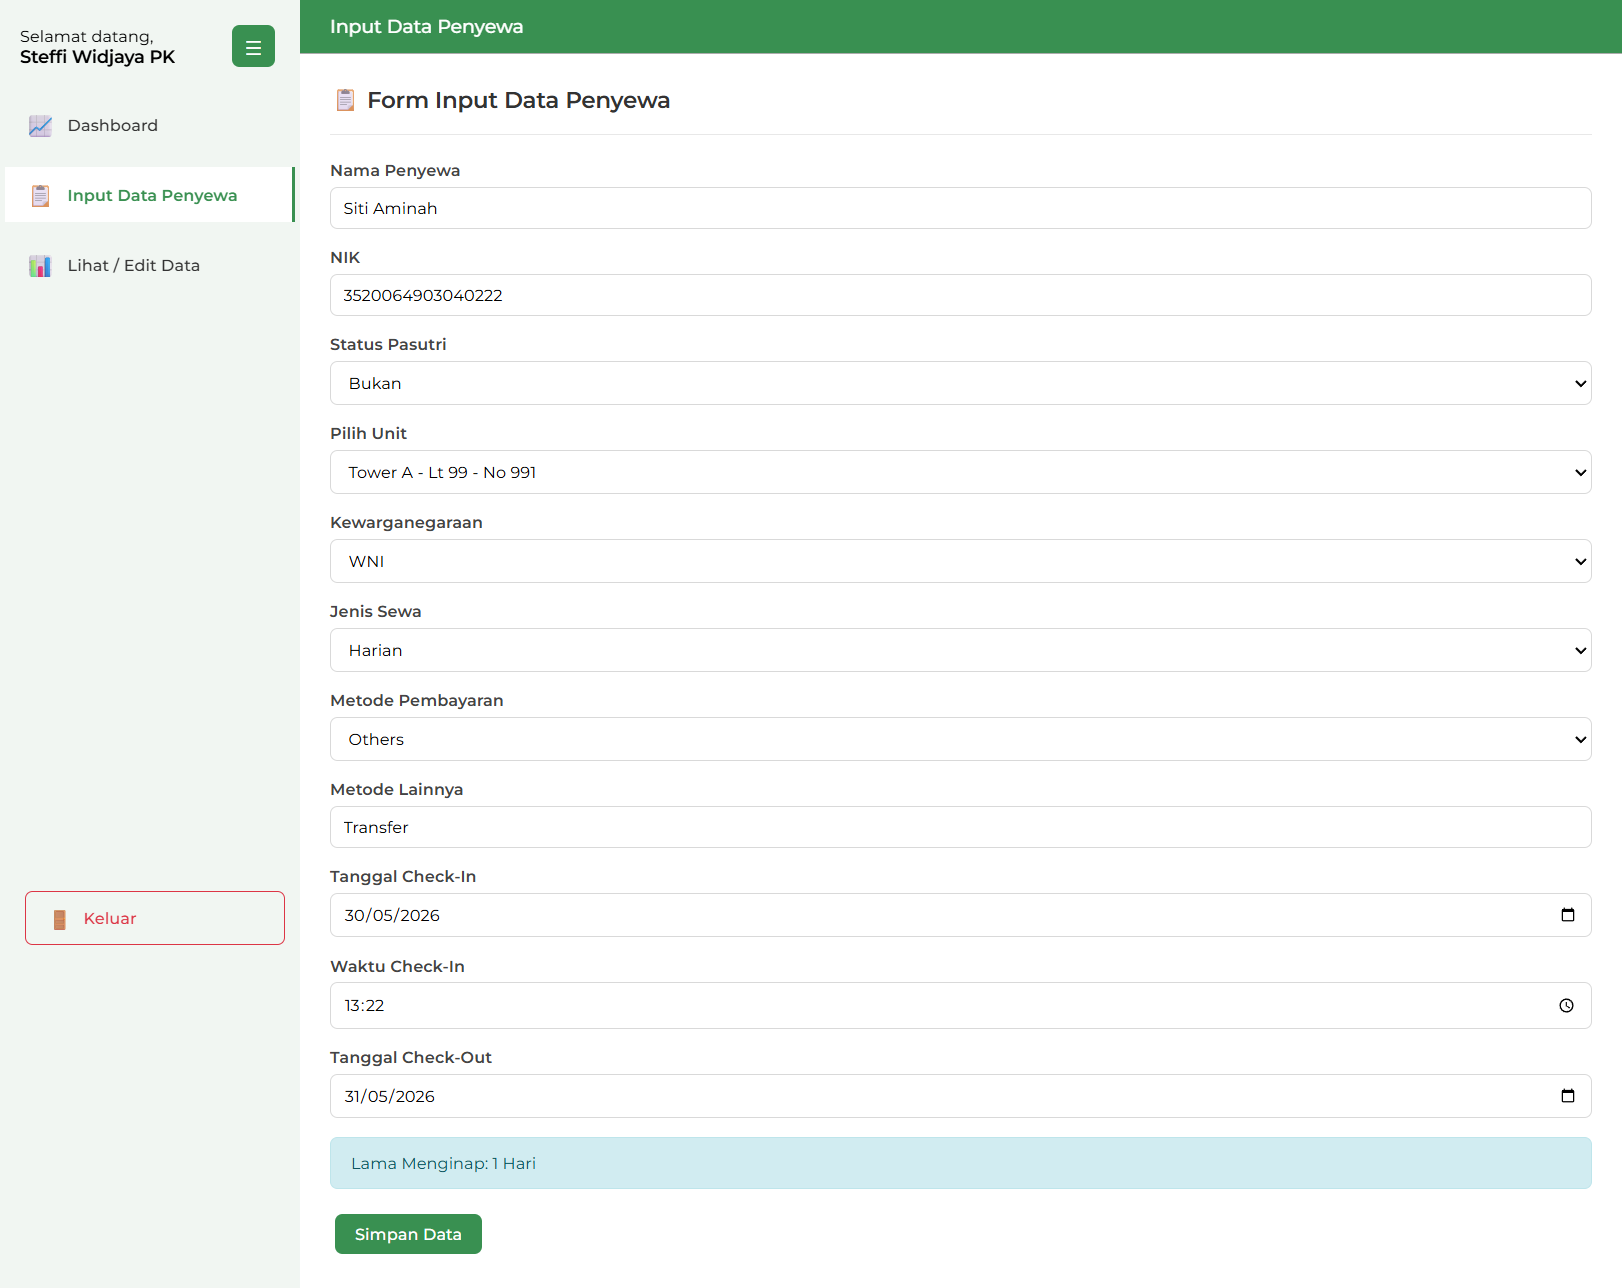
\includegraphics[width=0.7\textwidth]{Gambar/NONmelanggar2a.png} \\
    \vspace{0.2cm}
    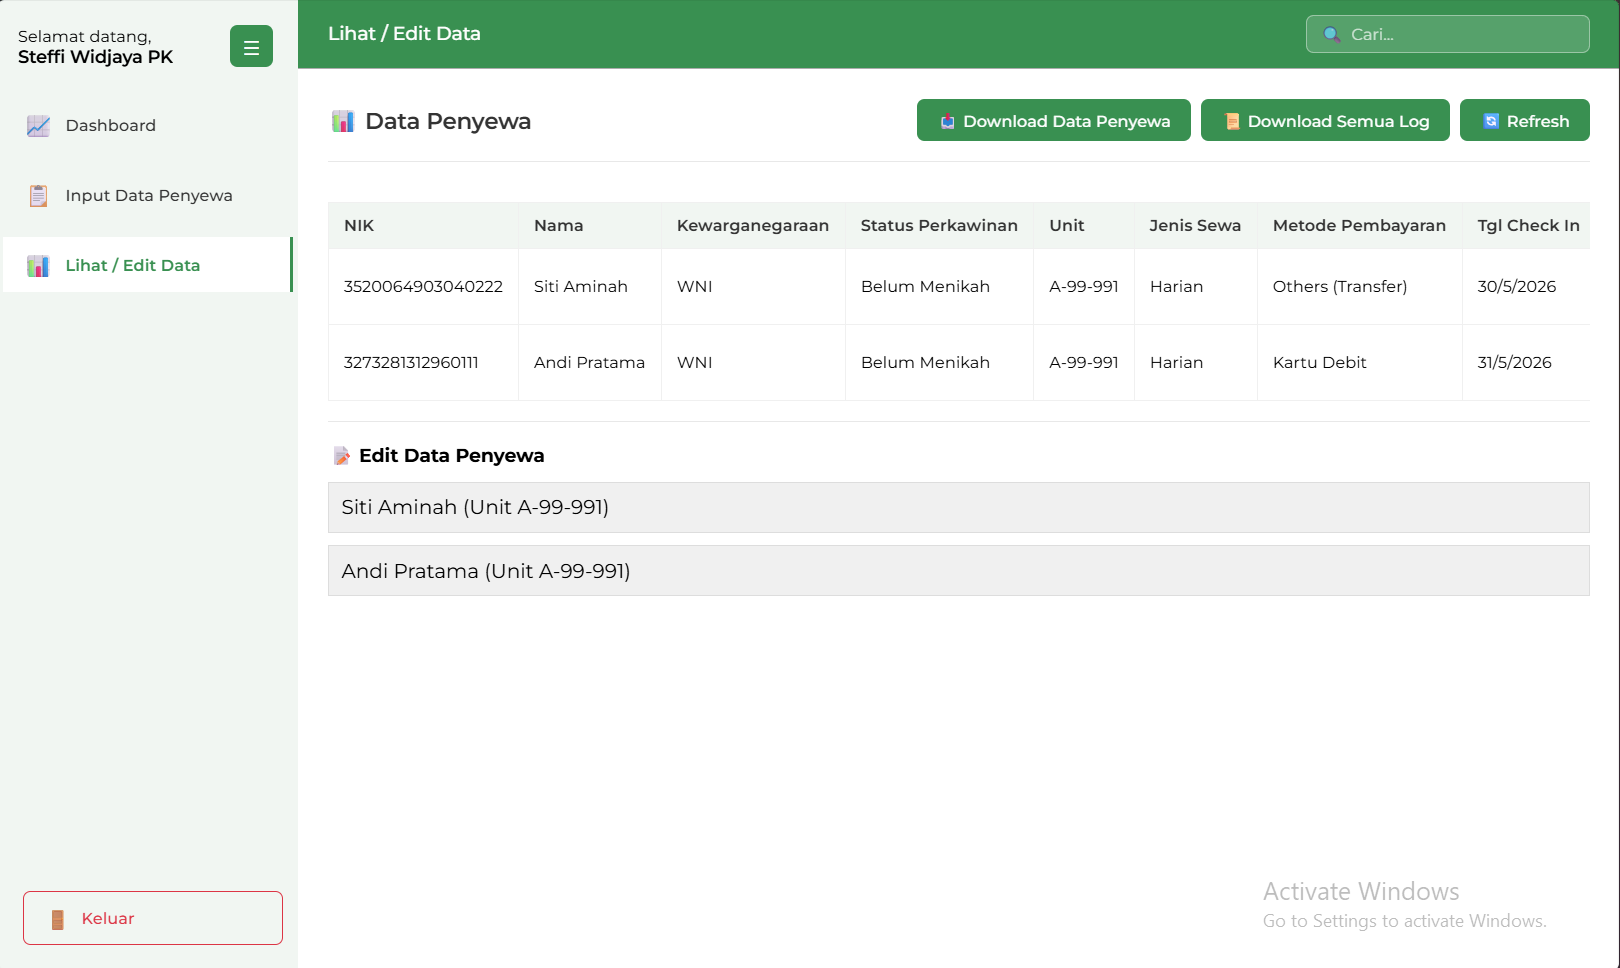
\includegraphics[width=0.7\textwidth]{Gambar/NONmelanggar2b.png}
    \caption{Simulasi Input Data Penyewa Normal (2)}
    \label{fig:sim_input_normal2}
\end{figure}

\begin{figure}[H]
    \centering
    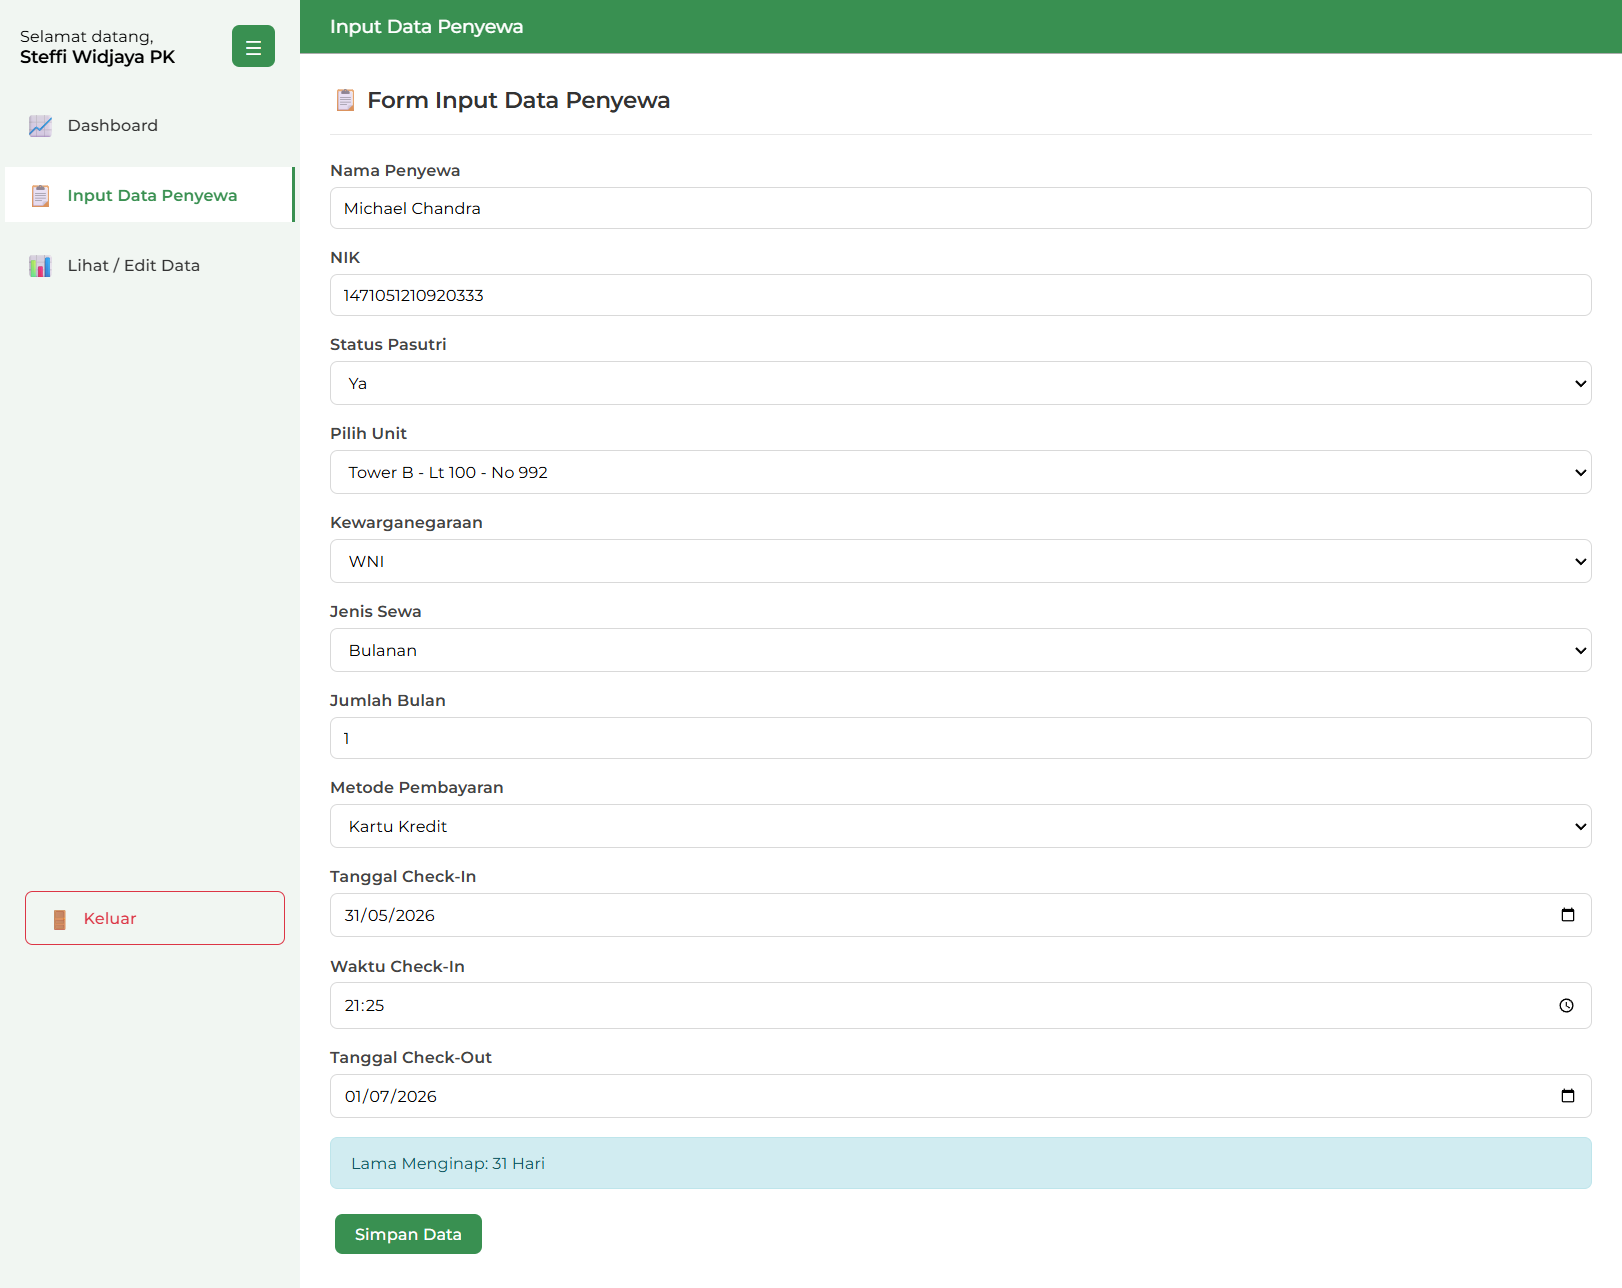
\includegraphics[width=0.7\textwidth]{Gambar/NONmelanggar3a.png} \\
    \vspace{0.2cm}
    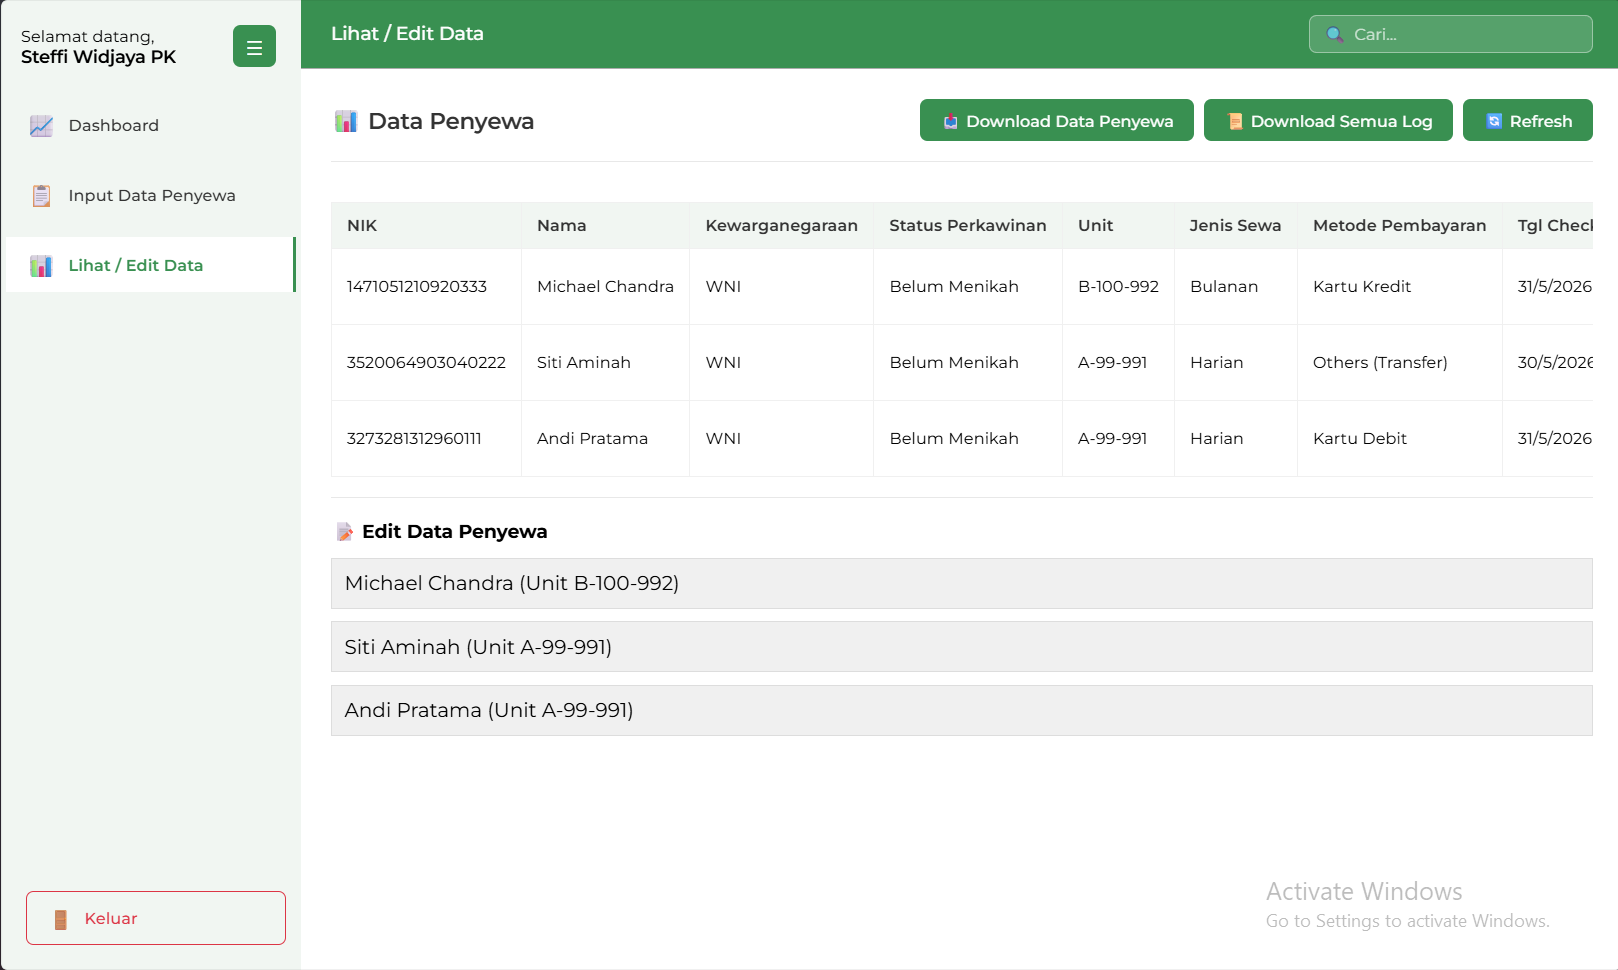
\includegraphics[width=0.7\textwidth]{Gambar/NONmelanggar3b.png}
    \caption{Simulasi Input Data Penyewa Normal (3)}
    \label{fig:sim_input_normal3}
\end{figure}

Gambar~\ref{fig:sim_input_normal1}, \ref{fig:sim_input_normal2}, dan \ref{fig:sim_input_normal3} memperlihatkan pengisian data dengan karakteristik penyewa normal. Parameter yang diinputkan merepresentasikan ciri transaksi yang minim risiko, seperti pemilihan durasi menginap jangka menengah hingga panjang serta kedatangan pada rentang waktu operasional yang wajar. Setelah seluruh kolom formulir dipastikan terisi dengan lengkap, pengguna klik tombol \textit{Simpan Data}. Aplikasi kemudian mengeksekusi data tersebut ke dalam model klasifikasi. Karena profil transaksi yang dikirimkan terindikasi aman (terklasifikasi ke dalam kelas 0), aplikasi memproses dan menyimpan data tersebut langsung ke dalam basis data, tanpa memunculkan notifikasi peringatan apa pun pada layar antarmuka pengguna.

\newpage
\subsection{Skenario Input Data Penyewa Tidak Normal}
Skenario kedua mendemonstrasikan pengisian formulir untuk profil penyewa yang terindikasi memiliki potensi pelanggaran aturan. Sama halnya dengan skenario sebelumnya, pengguna menginputkan informasi identitas dan detail transaksi ke dalam formulir pendataan.

\begin{figure}[H]
    \centering
    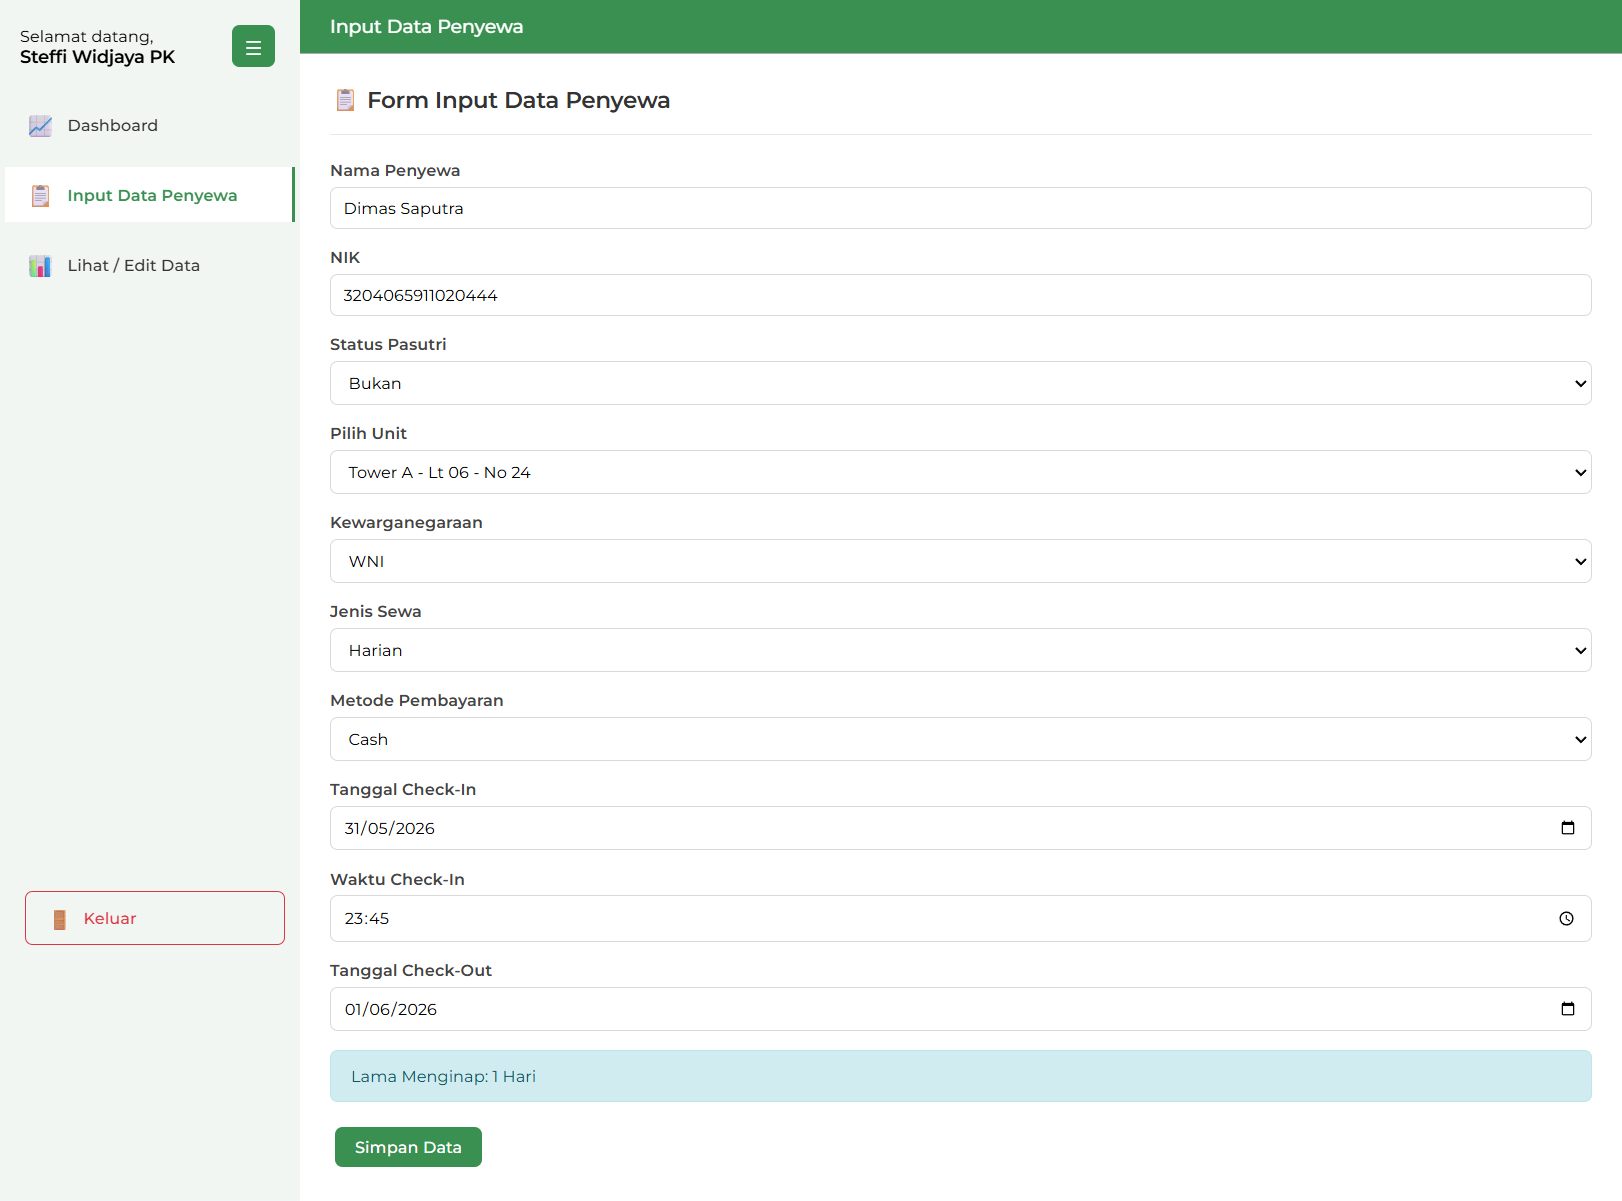
\includegraphics[width=0.7\textwidth]{Gambar/melanggar1a.png} \\
    \vspace{0.2cm}
    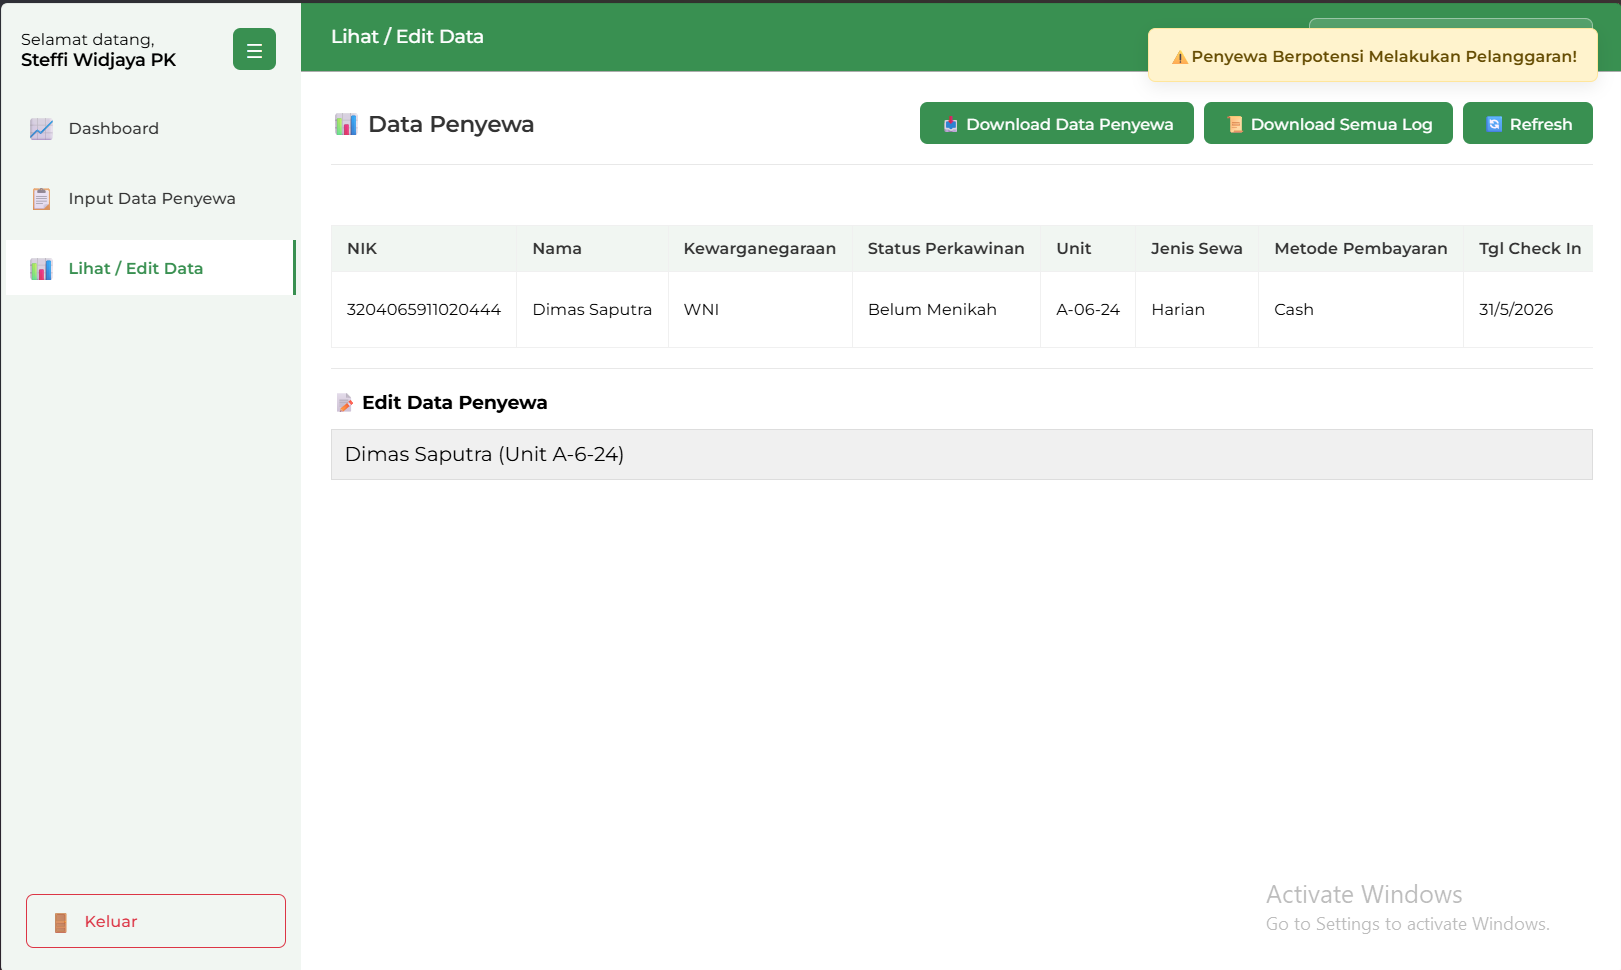
\includegraphics[width=0.7\textwidth]{Gambar/melanggar1b.png}
    \caption{Simulasi Input Data Penyewa Tidak Normal (1)}
    \label{fig:sim_input_tidak_normal1}
\end{figure}

\begin{figure}[H]
    \centering
    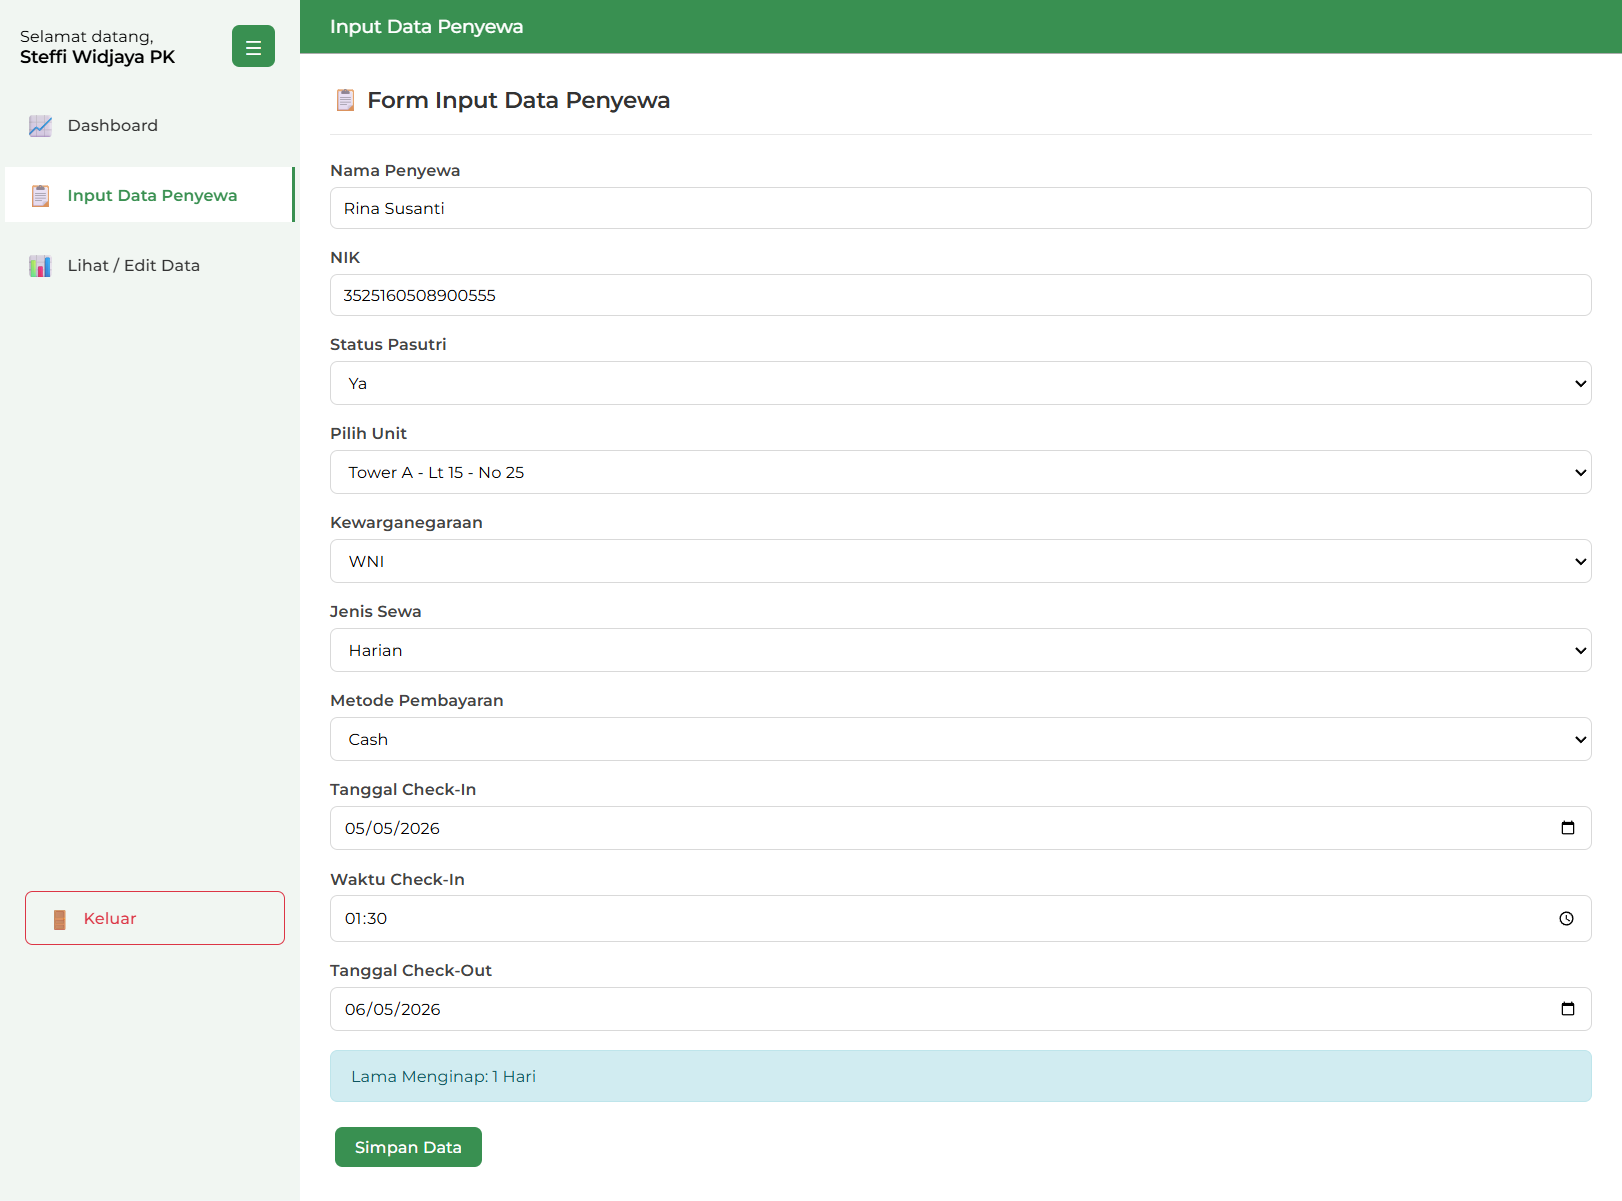
\includegraphics[width=0.7\textwidth]{Gambar/melanggar2a.png} \\
    \vspace{0.2cm}
    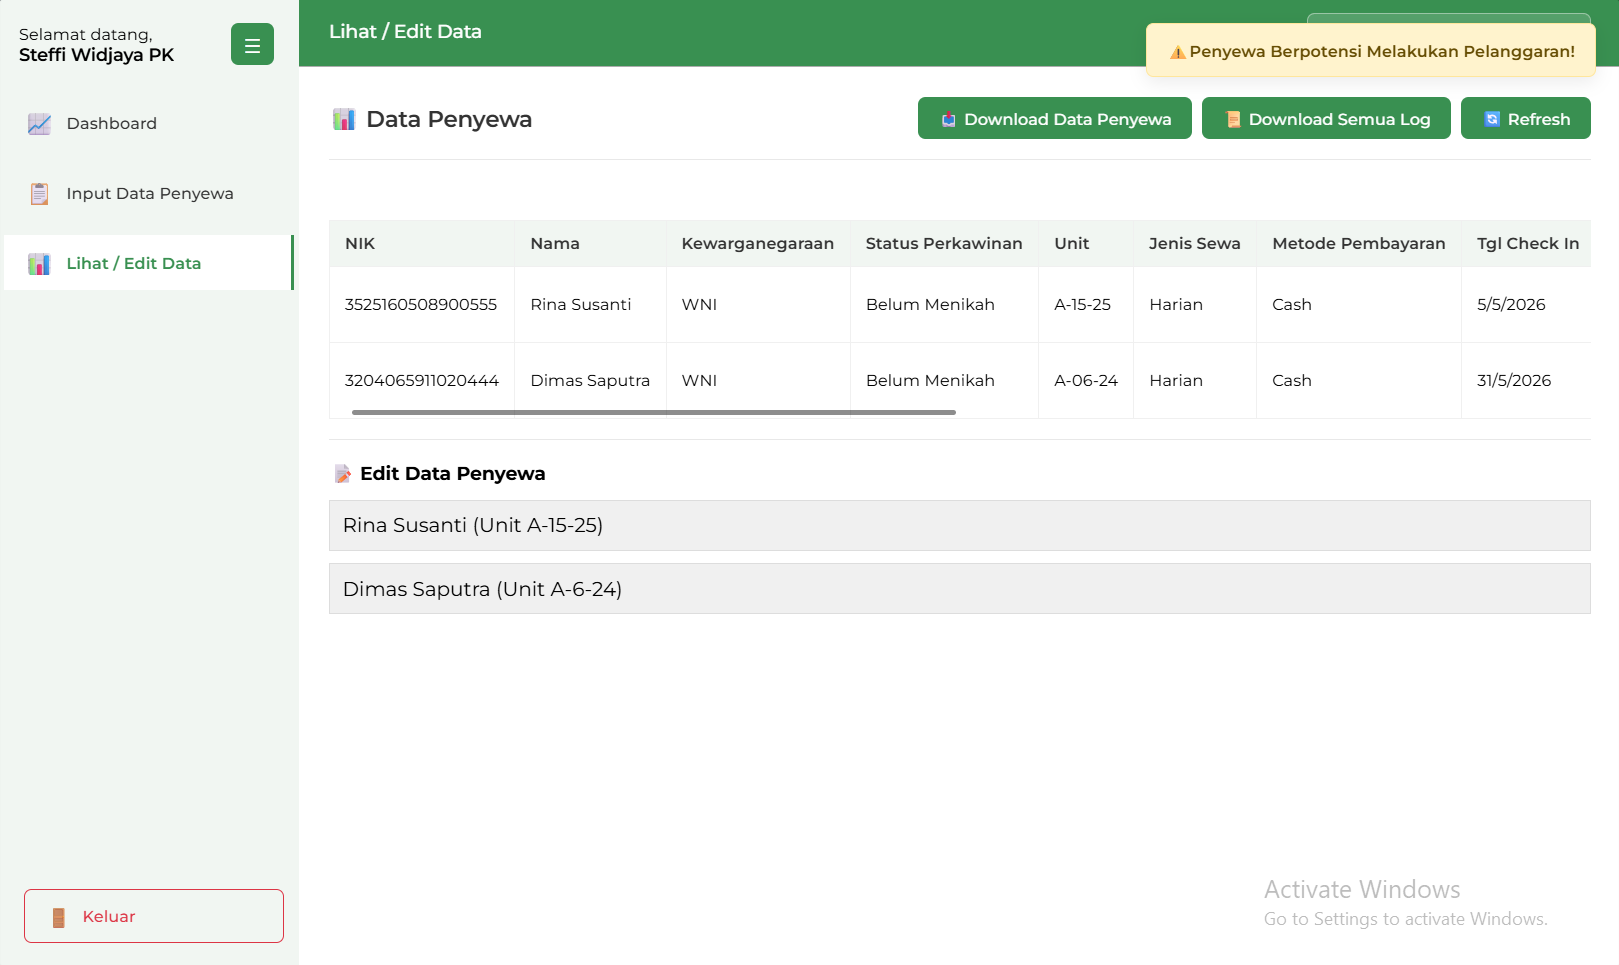
\includegraphics[width=0.7\textwidth]{Gambar/melanggar2b.png}
    \caption{Simulasi Input Data Penyewa Tidak Normal (2)}
    \label{fig:sim_input_tidak_normal2}
\end{figure}

\begin{figure}[H]
    \centering
    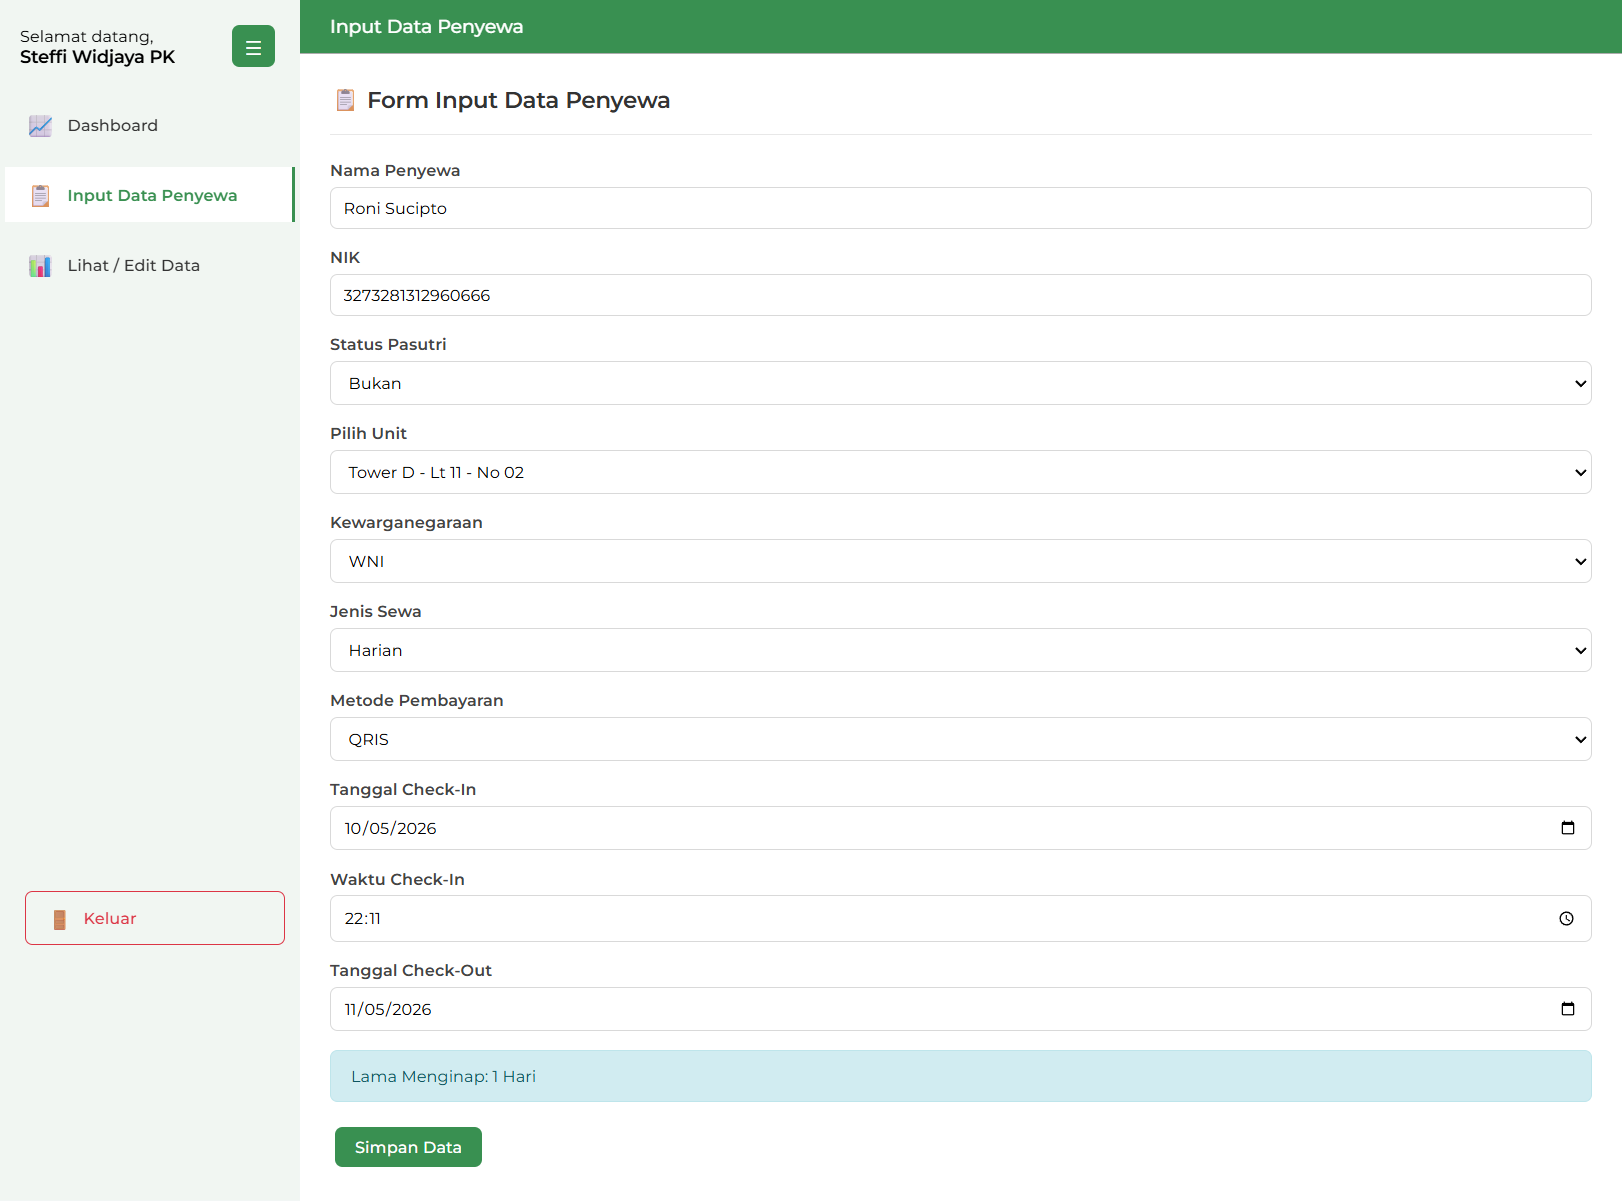
\includegraphics[width=0.7\textwidth]{Gambar/melanggar3a.png} \\
    \vspace{0.2cm}
    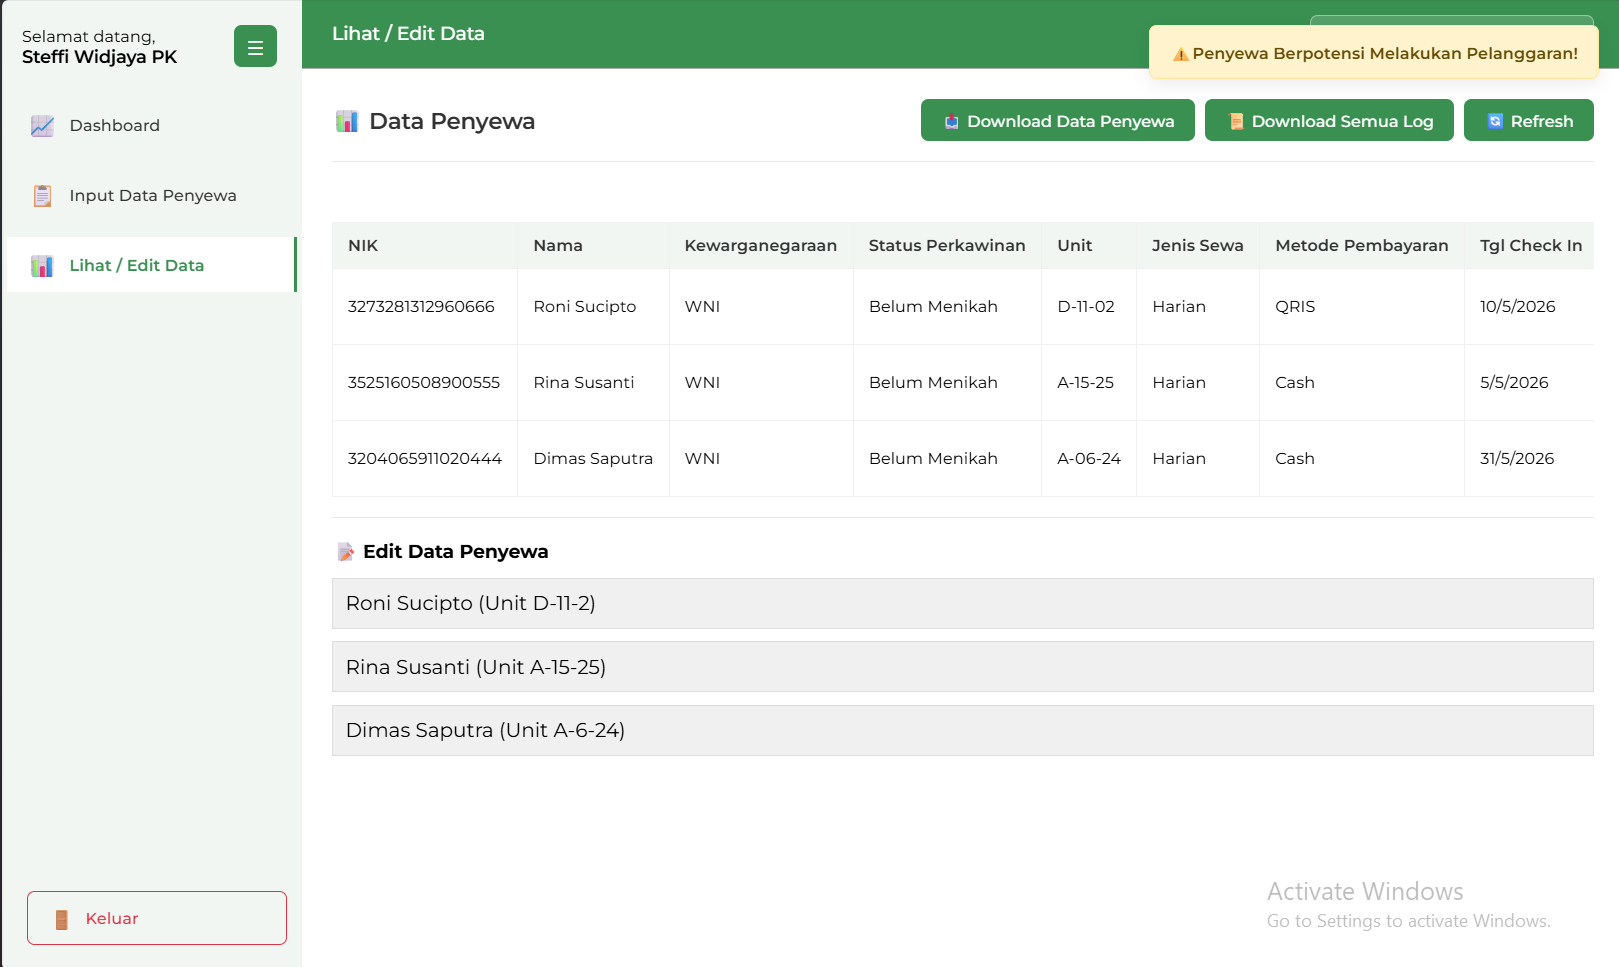
\includegraphics[width=0.7\textwidth]{Gambar/melanggar3b.png}
    \caption{Simulasi Input Data Penyewa Tidak Normal (3)}
    \label{fig:sim_input_tidak_normal3}
\end{figure}
\vspace{-0.5cm}
Gambar~\ref{fig:sim_input_tidak_normal1}, \ref{fig:sim_input_tidak_normal2}, dan \ref{fig:sim_input_tidak_normal3} memperlihatkan simulasi masukan data yang mengandung pola anomali. Penekanan pengisian difokuskan pada kombinasi atribut yang secara empiris menjadi karakteristik utama penyewa bermasalah pada tahapan analisis sebelumnya, seperti pemilihan jenis sewa harian yang dipadukan dengan durasi menginap yang sangat singkat (berkisar antara 0 hingga 1 hari). Setelah pengguna klik tombol \textit{Simpan Data}, aplikasi secara \textit{real-time} mentransmisikan sekumpulan data tersebut ke dalam model klasifikasi. Karena profil tersebut terdeteksi menyerupai karakteristik riwayat pelanggaran (terklasifikasi ke dalam kelas 1), maka aplikasi memberikan notifikasi berbunyi ``Penyewa Berpotensi Melakukan Pelanggaran!''. Peringatan ini bertujuan untuk langsung meningkatkan kewaspadaan Pengelola maupun Pelaku Komersil terhadap penyewa yang bersangkutan.


\subsection{Kesimpulan Hasil Pengujian}
Berdasarkan seluruh rangkaian pengujian fungsional aplikasi, pengujian integrasi, serta pengujian skenario peluncuran model di atas, dapat disimpulkan bahwa seluruh tahapan pengujian dan validasi sistem telah terlaksana dengan tuntas dan berjalan sesuai perancangan. Integrasi antara antarmuka aplikasi {data capture} dan model prediktif terbukti berfungsi secara optimal. Aplikasi mampu membaca, mengekstraksi, dan memproses setiap atribut data masukan pengguna secara \textit{real-time} untuk kemudian dianalisis oleh model klasifikasi secara akurat. Kepastian respons aplikasi yang presisi—berupa penyimpanan operasional yang mulus untuk profil aman serta intervensi notifikasi secara {\it real-time} untuk profil berisiko—menandakan bahwa seluruh fungsionalitas dan fitur pendeteksi dini (\textit{early warning system}) telah tervalidasi penuh serta siap dioperasikan sebagai instrumen pengawasan preventif pada kegiatan operasional penyewaan unit.